% Options for packages loaded elsewhere
\PassOptionsToPackage{unicode}{hyperref}
\PassOptionsToPackage{hyphens}{url}
%
\documentclass[
  ignorenonframetext,
]{beamer}
\title{Employee attrition}
\author{Mallikarjun Tilak}
\date{1/9/2022}

\usepackage{pgfpages}
\setbeamertemplate{caption}[numbered]
\setbeamertemplate{caption label separator}{: }
\setbeamercolor{caption name}{fg=normal text.fg}
\beamertemplatenavigationsymbolsempty
% Prevent slide breaks in the middle of a paragraph
\widowpenalties 1 10000
\raggedbottom
\setbeamertemplate{part page}{
  \centering
  \begin{beamercolorbox}[sep=16pt,center]{part title}
    \usebeamerfont{part title}\insertpart\par
  \end{beamercolorbox}
}
\setbeamertemplate{section page}{
  \centering
  \begin{beamercolorbox}[sep=12pt,center]{part title}
    \usebeamerfont{section title}\insertsection\par
  \end{beamercolorbox}
}
\setbeamertemplate{subsection page}{
  \centering
  \begin{beamercolorbox}[sep=8pt,center]{part title}
    \usebeamerfont{subsection title}\insertsubsection\par
  \end{beamercolorbox}
}
\AtBeginPart{
  \frame{\partpage}
}
\AtBeginSection{
  \ifbibliography
  \else
    \frame{\sectionpage}
  \fi
}
\AtBeginSubsection{
  \frame{\subsectionpage}
}
\usepackage{amsmath,amssymb}
\usepackage{lmodern}
\usepackage{iftex}
\ifPDFTeX
  \usepackage[T1]{fontenc}
  \usepackage[utf8]{inputenc}
  \usepackage{textcomp} % provide euro and other symbols
\else % if luatex or xetex
  \usepackage{unicode-math}
  \defaultfontfeatures{Scale=MatchLowercase}
  \defaultfontfeatures[\rmfamily]{Ligatures=TeX,Scale=1}
\fi
% Use upquote if available, for straight quotes in verbatim environments
\IfFileExists{upquote.sty}{\usepackage{upquote}}{}
\IfFileExists{microtype.sty}{% use microtype if available
  \usepackage[]{microtype}
  \UseMicrotypeSet[protrusion]{basicmath} % disable protrusion for tt fonts
}{}
\makeatletter
\@ifundefined{KOMAClassName}{% if non-KOMA class
  \IfFileExists{parskip.sty}{%
    \usepackage{parskip}
  }{% else
    \setlength{\parindent}{0pt}
    \setlength{\parskip}{6pt plus 2pt minus 1pt}}
}{% if KOMA class
  \KOMAoptions{parskip=half}}
\makeatother
\usepackage{xcolor}
\IfFileExists{xurl.sty}{\usepackage{xurl}}{} % add URL line breaks if available
\IfFileExists{bookmark.sty}{\usepackage{bookmark}}{\usepackage{hyperref}}
\hypersetup{
  pdftitle={Employee attrition},
  pdfauthor={Mallikarjun Tilak},
  hidelinks,
  pdfcreator={LaTeX via pandoc}}
\urlstyle{same} % disable monospaced font for URLs
\newif\ifbibliography
\usepackage{graphicx}
\makeatletter
\def\maxwidth{\ifdim\Gin@nat@width>\linewidth\linewidth\else\Gin@nat@width\fi}
\def\maxheight{\ifdim\Gin@nat@height>\textheight\textheight\else\Gin@nat@height\fi}
\makeatother
% Scale images if necessary, so that they will not overflow the page
% margins by default, and it is still possible to overwrite the defaults
% using explicit options in \includegraphics[width, height, ...]{}
\setkeys{Gin}{width=\maxwidth,height=\maxheight,keepaspectratio}
% Set default figure placement to htbp
\makeatletter
\def\fps@figure{htbp}
\makeatother
\setlength{\emergencystretch}{3em} % prevent overfull lines
\providecommand{\tightlist}{%
  \setlength{\itemsep}{0pt}\setlength{\parskip}{0pt}}
\setcounter{secnumdepth}{-\maxdimen} % remove section numbering
\ifLuaTeX
  \usepackage{selnolig}  % disable illegal ligatures
\fi

\begin{document}
\frame{\titlepage}

\begin{frame}{R Markdown}
\protect\hypertarget{r-markdown}{}
\end{frame}

\begin{frame}[fragile]{R Markdown}
\protect\hypertarget{r-markdown-1}{}
This is an R Markdown document. Markdown is a simple formatting syntax
for authoring HTML, PDF, and MS Word documents. For more details on
using R Markdown see \url{http://rmarkdown.rstudio.com}.

Installing required libraries

\begin{verbatim}
## -- Attaching packages --------------------------------------- tidyverse 1.3.1 --
\end{verbatim}

\begin{verbatim}
## v ggplot2 3.3.5     v purrr   0.3.4
## v tibble  3.1.6     v dplyr   1.0.7
## v tidyr   1.1.4     v stringr 1.4.0
## v readr   2.1.0     v forcats 0.5.1
\end{verbatim}

\begin{verbatim}
## -- Conflicts ------------------------------------------ tidyverse_conflicts() --
## x dplyr::filter() masks stats::filter()
## x dplyr::lag()    masks stats::lag()
\end{verbatim}

\begin{verbatim}
## 
## Attaching package: 'mice'
\end{verbatim}

\begin{verbatim}
## The following object is masked from 'package:stats':
## 
##     filter
\end{verbatim}

\begin{verbatim}
## The following objects are masked from 'package:base':
## 
##     cbind, rbind
\end{verbatim}

\begin{verbatim}
## Loading required package: lattice
\end{verbatim}

\begin{verbatim}
## 
## Attaching package: 'caret'
\end{verbatim}

\begin{verbatim}
## The following object is masked from 'package:purrr':
## 
##     lift
\end{verbatim}

\begin{verbatim}
## Registered S3 method overwritten by 'tree':
##   method     from
##   print.tree cli
\end{verbatim}

\begin{verbatim}
## randomForest 4.6-14
\end{verbatim}

\begin{verbatim}
## Type rfNews() to see new features/changes/bug fixes.
\end{verbatim}

\begin{verbatim}
## 
## Attaching package: 'randomForest'
\end{verbatim}

\begin{verbatim}
## The following object is masked from 'package:dplyr':
## 
##     combine
\end{verbatim}

\begin{verbatim}
## The following object is masked from 'package:ggplot2':
## 
##     margin
\end{verbatim}

\begin{verbatim}
## 
## Attaching package: 'xgboost'
\end{verbatim}

\begin{verbatim}
## The following object is masked from 'package:dplyr':
## 
##     slice
\end{verbatim}

Loading the data and checking for null or NA values

Date formatting of the variables associated with date

\#encoding target variable

\begin{verbatim}
##   Emp_ID     MMM.YY Age Gender City Education_Level Salary Dateofjoining
## 1      1 2016-03-01  28   Male  C23          Master  57387    2015-12-24
## 2      1 2016-01-01  28   Male  C23          Master  57387    2015-12-24
## 3      1 2016-02-01  28   Male  C23          Master  57387    2015-12-24
## 4      2 2017-11-01  31   Male   C7          Master  67016    2017-11-06
## 5      2 2017-12-01  31   Male   C7          Master  67016    2017-11-06
## 6      4 2017-03-01  43   Male  C13          Master  65603    2016-12-07
##   LastWorkingDate.x Joining.Designation Designation Total.Business.Value
## 1        2016-03-11                   1           1                    0
## 2              <NA>                   1           1              2381060
## 3              <NA>                   1           1              -665480
## 4              <NA>                   2           2                    0
## 5              <NA>                   2           2                    0
## 6              <NA>                   2           2               350000
##   Quarterly.Rating DaysInCompany lyd LastWorkingDate.y daysb4lastworkingdate
## 1                2       68 days Yes        2016-03-11               10 days
## 2                2        8 days  No        2016-03-11               70 days
## 3                2       39 days  No        2016-03-11               39 days
## 4                1        0 days  No              <NA>               NA days
## 5                1       25 days  No              <NA>               NA days
## 6                1       84 days  No        2017-04-27               57 days
##   attrition year month day
## 1       Yes 2016     3  01
## 2       Yes 2016     1  01
## 3       Yes 2016     2  01
## 4        No 2017    11  01
## 5        No 2017    12  01
## 6       Yes 2017     3  01
\end{verbatim}
\end{frame}

\begin{frame}[fragile]{USE different DATA for test}
\protect\hypertarget{use-different-data-for-test}{}
\begin{verbatim}
## # A tibble: 6 x 21
## # Groups:   Emp_ID [6]
##   Emp_ID MMM.YY       Age Gender City  Education_Level Salary Dateofjoining
##    <int> <date>     <int> <fct>  <fct> <fct>            <int> <date>       
## 1      2 2017-12-01    31 Male   C7    Master           67016 2017-11-06   
## 2      6 2017-12-01    31 Female C11   Bachelor         78728 2017-07-31   
## 3     11 2017-12-01    28 Female C19   Master           42172 2017-12-07   
## 4     14 2017-12-01    39 Female C26   College          19734 2017-10-16   
## 5     25 2017-12-01    31 Male   C24   Bachelor        102077 2014-10-30   
## 6     26 2017-12-01    43 Male   C14   Master          132577 2015-05-07   
## # ... with 13 more variables: LastWorkingDate.x <date>,
## #   Joining.Designation <int>, Designation <int>, Quarterly.Rating <int>,
## #   DaysInCompany <drtn>, lyd <chr>, LastWorkingDate.y <date>,
## #   daysb4lastworkingdate <drtn>, attrition <fct>, year <chr>, month <dbl>,
## #   day <chr>, Total.Business.Value <int>
\end{verbatim}

\begin{verbatim}
##   Emp_ID     MMM.YY Age Gender City Education_Level Salary Dateofjoining
## 1      1 2016-03-01  28   Male  C23          Master  57387    2015-12-24
## 2      1 2016-01-01  28   Male  C23          Master  57387    2015-12-24
## 3      1 2016-02-01  28   Male  C23          Master  57387    2015-12-24
## 4      4 2017-03-01  43   Male  C13          Master  65603    2016-12-07
## 5      4 2017-02-01  43   Male  C13          Master  65603    2016-12-07
## 6      4 2017-01-01  43   Male  C13          Master  65603    2016-12-07
##   LastWorkingDate.x Joining.Designation Designation Total.Business.Value
## 1        2016-03-11                   1           1                    0
## 2              <NA>                   1           1              2381060
## 3              <NA>                   1           1              -665480
## 4              <NA>                   2           2               350000
## 5              <NA>                   2           2                    0
## 6              <NA>                   2           2                    0
##   Quarterly.Rating DaysInCompany lyd LastWorkingDate.y daysb4lastworkingdate
## 1                2       68 days Yes        2016-03-11               10 days
## 2                2        8 days  No        2016-03-11               70 days
## 3                2       39 days  No        2016-03-11               39 days
## 4                1       84 days  No        2017-04-27               57 days
## 5                1       56 days  No        2017-04-27               85 days
## 6                1       25 days  No        2017-04-27              116 days
##   attrition year month day
## 1       Yes 2016     3  01
## 2       Yes 2016     1  01
## 3       Yes 2016     2  01
## 4       Yes 2017     3  01
## 5       Yes 2017     2  01
## 6       Yes 2017     1  01
\end{verbatim}

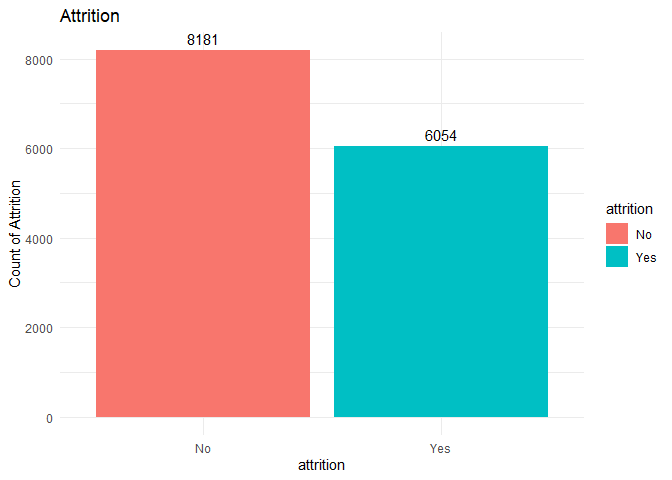
\includegraphics{Figs/plot1-1.png}

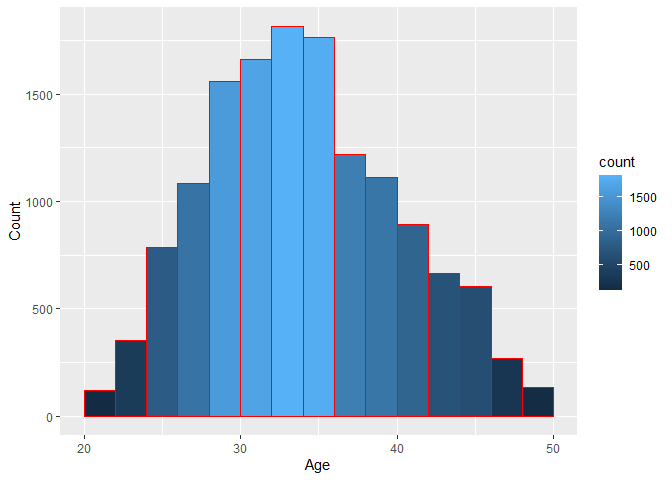
\includegraphics{Figs/plot2-1.png} 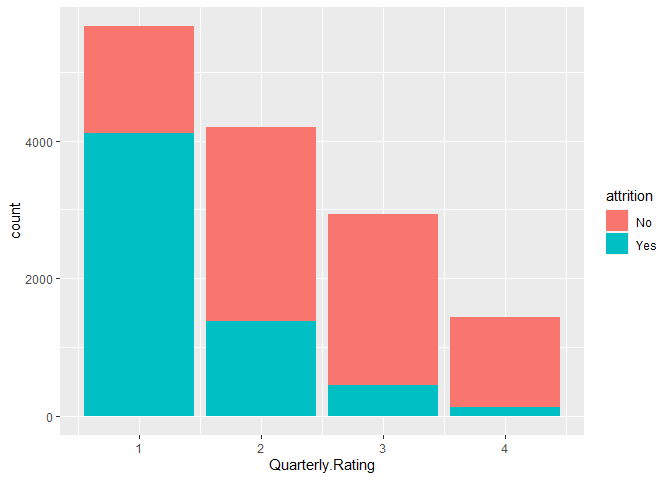
\includegraphics{Figs/plot2-2.png}
\#\# variation of attrition w.r.t. education and income

\begin{verbatim}
## `summarise()` has grouped output by 'Education_Level'. You can override using the `.groups` argument.
\end{verbatim}

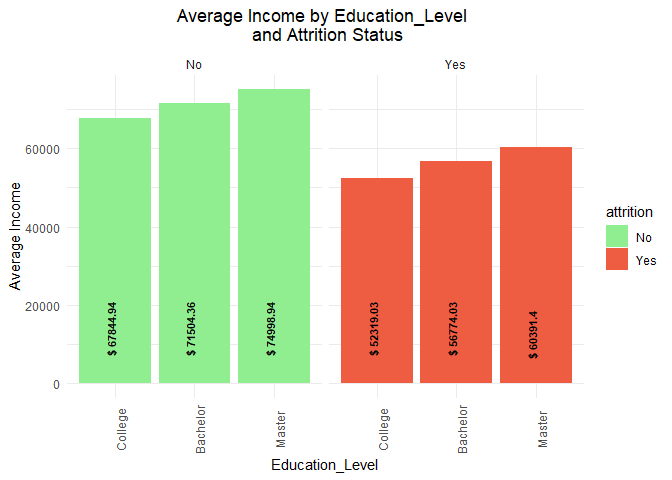
\includegraphics{Figs/correlogram-1.png}
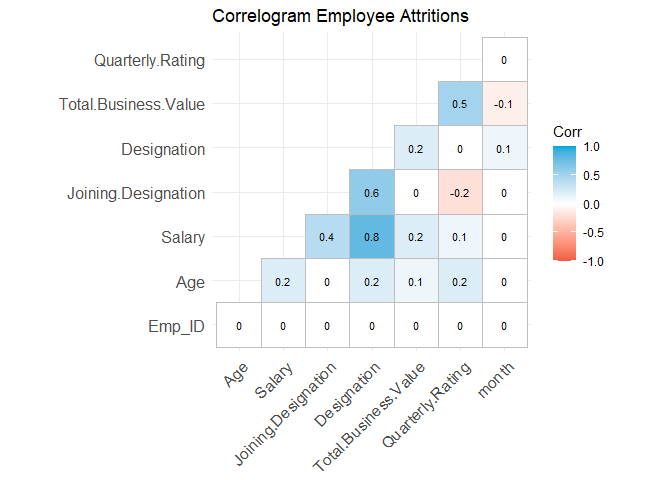
\includegraphics{Figs/correlogram-2.png} \#\# Remove unwanted colum

\#\#\%\%\%\%XG BOOST\%\%

\begin{block}{One hot Encoding for df}
\protect\hypertarget{one-hot-encoding-for-df}{}
\#converting to Dmatrix

\begin{verbatim}
## [13:36:52] WARNING: amalgamation/../src/learner.cc:1115: Starting in XGBoost 1.3.0, the default evaluation metric used with the objective 'binary:logistic' was changed from 'error' to 'logloss'. Explicitly set eval_metric if you'd like to restore the old behavior.
## [1]  train-logloss:0.594290 
## [2]  train-logloss:0.538056 
## [3]  train-logloss:0.503478 
## [4]  train-logloss:0.480051 
## [5]  train-logloss:0.463478 
## [6]  train-logloss:0.451242 
## [7]  train-logloss:0.442515 
## [8]  train-logloss:0.432905 
## [9]  train-logloss:0.425032 
## [10] train-logloss:0.419400 
## [11] train-logloss:0.414647 
## [12] train-logloss:0.409879 
## [13] train-logloss:0.404354 
## [14] train-logloss:0.400843 
## [15] train-logloss:0.397112 
## [16] train-logloss:0.394142 
## [17] train-logloss:0.387689 
## [18] train-logloss:0.383489 
## [19] train-logloss:0.376327 
## [20] train-logloss:0.371369
\end{verbatim}

\begin{verbatim}
## [1] "test-error= 0.365721997300945"
\end{verbatim}

\#confusion matrix 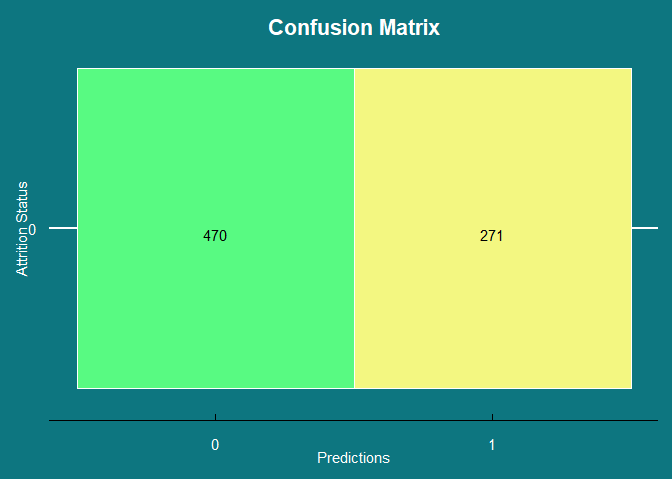
\includegraphics{Figs/cnfmatrix-1.png} The test cases
were chosen such that all of them were belonging to `0' label
\end{block}
\end{frame}

\end{document}
